\begin{enumerate}[label=\thesubsection.\arabic*.,ref=\thesubsection.\theenumi]
\numberwithin{equation}{enumi}

\item Find the closed loop transfer function for the system in Fig. \label{fig:ee18btech11035_block} given that
\begin{align}
\label{eq:ee18btech11035_G(s)}
G\brak{s}=\frac{1}{s^2+2s}
\end{align}
%
\begin{figure}[!ht]
    \begin{center}
		\resizebox{\columnwidth}{!}{\tikzset{
        block/.style = {draw, rectangle,
            minimum height=1cm,
            minimum width=2cm},
        input/.style = {coordinate,node distance=1cm},
        output/.style = {coordinate,node distance=4cm},
        arrow/.style={draw, -latex,node distance=2cm},
        pinstyle/.style = {pin edge={latex-, black,node distance=2cm}},
        sum/.style = {draw, circle, node distance=1cm},
}

\begin{tikzpicture}[node distance=2.5cm,auto,>=latex']
  \node [input, name=input] {};
  \node [sum, right of=input] (sum) {};
  \node [block, right of = sum] (block1) {$k$};
  \node [block, right of = block1] (block2) {$G(s)$};
  \node [output, right of= block2] (output) {};
  \draw [->] (input) -- node {$r$} (sum);
  \draw [->] (sum) -- node {} (block1);
  \draw [->] (block1) -- node {} (block2);
  \draw [->] (block2) -- node [name =y] {$y$} (output);
  \draw [->] (y) -- ++ (0,-2) -| node [pos=0.99] {$-$} (sum);
\end{tikzpicture}}
	\end{center}
\caption{}
\label{fig:ee18btech11035_block}
\end{figure}
\\
\solution The closed loop transfer function is
\begin{align}
H\brak{s} &= \frac{kG\brak{s}}{1+kG\brak{s}}
\label{eq:ee18btech11035_4}
\\
 &= \frac{k}{s^2+2s+k}
\label{eq:ee18btech11035_H(s)}
\end{align}
after substituting from \eqref{eq:ee18btech11035_G(s)}.
\item Find the step response of the system.\\
\solution The characteristics of the poles of transfer function describes the property of the transfer function.\\
Calculating poles :
\begin{align}
    s^2+2s+k&=0\\
    s&=\frac{-2\pm\sqrt{\brak{-2}^2-4\brak{1}\brak{k}}}{2\brak{1}}\\
    \label{ee18btech11035_poles}
    s&=-1\pm\sqrt{1-k}
\end{align}

Over Damped System:\\
For the closed loop transfer function \eqref{eq:ee18btech11035_H(s)} to be Over damped system,poles should be Real and Distinct.\\
As poles are Real and Distinct $k$ should be less than 1\\
Considering k=0.5\\
\begin{align}
H\brak{s} &= \frac{0.5}{s^2+2s+0.5}
\end{align}
after substituting from \eqref{eq:ee18btech11035_H(s)}.
From \eqref{ee18btech11035_poles}
\begin{align}
s&=-1\pm\sqrt{0.5}
\end{align}
Poles are at \(-1+\frac{1}{\sqrt{2}} ,-1-\frac{1}{\sqrt{2}}\)\\
Calculating Step response
\begin{align}
X\brak{s}&=\frac{1}{s}\\
Y\brak{s}&=H\brak{s}X\brak{s}\\
&=\frac{0.5}{s^2+2s+0.5}\frac{1}{s}
\end{align}
\begin{multline}
    y\brak{t}&=\brak{{1-e^{-t}\cosh{\brak{\frac{t}{\sqrt{2}}}}-\sqrt{2}e^{-t}\sinh{\brak{\frac{t}{\sqrt{2}}}}}}u\brak{t}
\end{multline}
    
Under Damped System:\\
For the closed loop transfer function \eqref{eq:ee18btech11035_H(s)} to be Under damped system,poles should be Complex and Conjugate.\\
As poles are Complex and Conjugate $k$ should be greater than 1\\
Considering k=2\\
\begin{align}
H\brak{s} &= \frac{2}{s^2+2s+2}
\end{align}
after substituting from \eqref{eq:ee18btech11035_H(s)}.
From \eqref{ee18btech11035_poles}
\begin{align}
s&=-1\pm\iota
\end{align}
Poles are at -1+\(\iota\),-1-\(\iota\)\\
Calculating Step response
\begin{align}
X\brak{s}&=\frac{1}{s}\\
Y\brak{s}&=H\brak{s}X\brak{s}\\
&=\frac{2}{s^2+2s+2}\frac{1}{s}\\
y\brak{t}&=\brak{1-e^{-t}\cos{t}-e^{-t}\sin{t}}u\brak{t}
\end{align}


Critical Damped System:\\
For the closed loop transfer function \eqref{eq:ee18btech11035_H(s)} to be Critical damped system,poles should be Real at same location.\\
As poles are Real and equal $k$ should be 1\\
\begin{align}
H\brak{s} &= \frac{1}{s^2+2s+1}
\end{align}
after substituting from \eqref{eq:ee18btech11035_H(s)}.
From \eqref{ee18btech11035_poles}
\begin{align}
s&=-1
\end{align}
Pole is at -1 and it is a second order pole.\\
Calculating Step response
\begin{align}
X\brak{s}&=\frac{1}{s}\\
Y\brak{s}&=H\brak{s}X\brak{s}\\
&=\frac{1}{s^2+2s+1}\frac{1}{s}\\
y\brak{t}&=\brak{1-e^{-t}-te^{-t}}u\brak{t}
\end{align}

\item  Find $k$ in  such that the step response of the closed-loop system has minimum settling time and have no overshoot.\\
\solution Settling time is defined as the time required for the transient's damped oscillations to
reach and stay within $\pm 2$\% of the steady-state value.\\
\begin{figure}[!h]
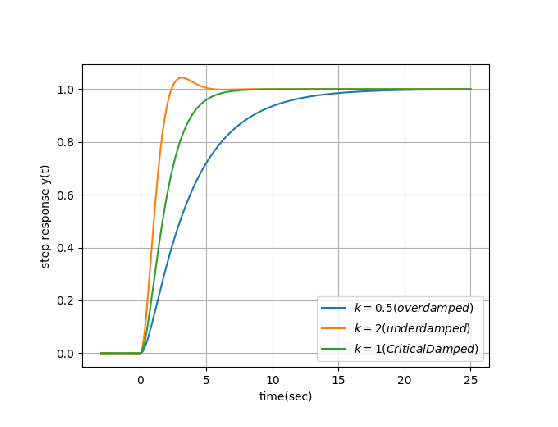
\includegraphics[width=\columnwidth]{./figures/ee18btech11035_4.eps}
\caption{Plot of step response of systems}
\label{fig:ee18btech11035_y(t)}
\end{figure}

Above plot justifies that critical damped system \brak{k=1} has minimum settling time and also doesn't overshoot.\\
Calculating Settling time\\
\begin{align}
    \label{eq:calculating_time}
    1-e^{-t}-te^{-t}&=0.98
\end{align}
Solving \eqref{eq:calculating_time} graphically\\
\begin{figure}[!h]
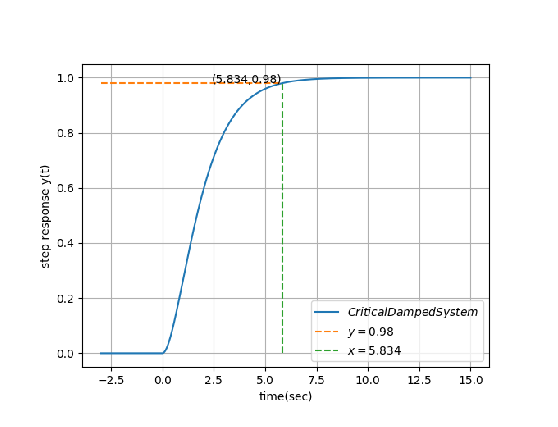
\includegraphics[width=\columnwidth]{./figures/ee18btech11035_5.eps}
\caption{}
\label{fig:ee18btech11035_settling}
\end{figure}

Therefore,Settling time is 0.584sec.
\end{enumerate}
